
%%%
% Any line that begins with a percent symbol is a comment. To compile
% this document and view the output:
%
% Run Latex
% Run Bibtex
% Then run Latex twice.
%
% This should produce the output PDF file named main.pdf
%%%

% This defines the style to use for this document.
% Do not modify.
\documentclass[letterpaper]{article}

% The following are akin to "import" statements in Python or Java -
% these import useful commands into the document for you to use.  You
% don't have to modify any of these lines. The AAAI package formats
% this document in the style of submissions to the American
% Association for Artificial Intelligence conference, one of the top
% AI conferences in the world. You will find that many academic
% publications in AI use this format.
\usepackage{aaai}
\usepackage{times}
\usepackage{helvet}
\usepackage{courier}
\setlength{\pdfpagewidth}{8.5in}
\setlength{\pdfpageheight}{11in}
\usepackage{amsmath}
\usepackage{amsthm}
\usepackage{graphicx}
\usepackage{graphics}
\usepackage{moreverb}
\usepackage{subfigure}
\usepackage{epsfig}
\usepackage{txfonts}
\usepackage{algpseudocode}
\usepackage{multirow, multicol}
\usepackage{url}
\usepackage{tablefootnote}
\usepackage{color}

\setcounter{secnumdepth}{1}
\nocopyright

% Fill in your paper title, names and emails below
% The "\\" is used to break lines. The \url command
% is useful for typesetting URLs and email addresses (it uses the
% Courier font).
\title{A Machine Learning Approach to Clothing Classification}
\author{Ian Rolls}\\

% This is the "true" start of the document. All the text in your
% write-up should be placed within the \begin{document} and
% \end{document} decorators.
\begin{document}

\maketitle % formats the title nicely, do not modify

% While at this point you could just begin your write-up, often, it's
% useful to write each section of your write-up in a separate tex
% file (not unlike the modular decomposition you do for code you
% write). These \input commands insert the contents of the
% specified tex files in the order specified. Every write-up you
% submit must contain the following sections, in the shown order. Open
% each of the indicated tex files to understand what goes in each
% section, as well as for more TeX tips.

% Place the contents of your abstract between the
% \begin{abstract} and \end{abstract} decorators.

\begin{abstract}

Classifying types of clothing is useful for clothing retailers, especially retailers with a digital presence who sell clothing online. Being able to automatically categorize items of clothing is useful for creating search options on an online platform for consumers to narrow down product searches. We develop a clothing classification model using logistic regression and k-nearest neighbor techniques. We conclude that using the k-nearest neighbors model with more advanced feature selection methods is the most accurate way to classify clothing labels without the use of neural networks.

% The \textbf{} command makes the specified text bold. The \emph{} or
% \textit{} command are used to italicize text. In general, text is never
% underlined.

% DON'T FORGET TO MATCH EACH OPEN BRACE WITH A CLOSING BRACE!
\end{abstract}



% The \section{} command formats and sets the title of this
% section. We'll deal with labels later.
\section{Introduction}
\label{sec:intro}

 Clothing classification is an extremely useful tool for e-commerce, as it could be used by companies to create filterable tags for their website, identify and sort clothing in a shipping warehouse, or to break out data by clothing category. This would replace the need for humans to manually classify items and could reduce a company's labor costs while increasing efficiency.

Recent work in the field of clothing classification utilizes neural networks, deep learning, and random forests to classify clothing in photos involving a human subject wearing a particular garment or garments. These techniques are needed to isolate the clothing from the person and the background to focus and identify the garment itself. Bossard et al. uses random forests as their primary classification tool, and had varying results based on what aspect of the clothing they were classifying. For "looks," the model had an accuracy of $\sim$72\% whereas the accuracy for "styles" had an accuracy of $\sim$37\% with the rest of the metrics somewhere in the middle \cite{eth_biwi_00974}. Zhou et al. uses a neural network model for clothing classification, notably using advanced feature extraction techniques to provide the model with relevant information. They train a separate neural network to extract features from a given image which makes for a more dynamic, generally applicable model that can process noisy images. The main neural network itself is relatively standard, including an L1 regularization and an optimization algorithm for improved gradient descent. Their model ended up with an F1 score of $\sim$0.93 \cite{Zhou}. Both papers use the exact same dataset and their feature extraction techniques are almost identical. This likely means that the neural network is a better learning model than the random forest model for predicting clothing labels.



% Citations: As you can see above, you create a citation by using the
% \cite{} command. Inside the braces, you provide a "key" that is
% uniue to the paper/book/resource you are citing. How do you
% associate a key with a specific paper? You do so in a separate bib
% file --- for this document, the bib file is called
% project1.bib. Open that file to continue reading...

% Note that merely hitting the "return" key will not start a new line
% in LaTeX. To break a line, you need to end it with \\. To begin a 
% new paragraph, end a line with \\, leave a blank
% line, and then start the next line (like in this example).



\section{Dataset}
\label{sec:dataset}
The data set we use for training our models is the Fashion MNIST, which was aggregated by Zalando, a clothing e-commerce website. Our dataset contains 70000 unique images of clothing, each represented as a 28x28 matrix containing a color value, represented in by a grey-scale value. Each of these color values is a feature in our model, which gives us 784 features in total.

 Each image also gets assigned a "label" value in the range of 0 to 9. Each number corresponds to the clothing category of the article shown in the image. These categories and their corresponding number values can be seen in table 1. Our target is the label, as our goal is to predict which category an article of clothing belongs to which category given an image. The number of images corresponding to each unique label is identical, so there are 7000 images for each of the 10 categories.

\begin{table}[!h]
    \centering
    \begin{tabular}{|c|c|}
        \hline
        Number & Catagory\\
        \hline
        0 & T-shirt/top\\
        1 & Trouser\\
        2 & Pullover\\
        3 & Dress\\
        4 & Coat\\
        5 & Sandal\\
        6 & Shirt\\
        7 & Sneaker\\
        8 & Bag\\
        9 & Ankle boot\\
        \hline
    \end{tabular}
    \caption{Label Catagories}
    \label{tab:my_label}
\end{table}

\section{Exploratory Analysis}
\label{sec:background}

We first performed a 6:1 train/test split on our data, giving us a dataset of 60000 images for the training data and 10000 images for the testing. This will allow us to test the model with data not seen in training to give us a true test of the accuracy. If the model over-fits our training data, this will show in the testing results, as it will not perform as well on unseen data.

One interesting aspect of the dataset is that some categories are very similar - so much so that an untrained human might have a hard time distinguishing between the two. Most notably, T-shirt/top and shirt are extremely similar categories. Secondly, pullover and coat also might be tricky to distinguish in some cases. We expect that the model might have a harder time distinguishing between these categories, especially because the 28x28 pixel images are low resolution and therefore might not be able to convey some distinctions (for example a pullover and a coat might look similar with the zipper as the exception). Figures 1 and 2 display what the 28x28 image looks like. As you can see, it would be difficult for a human to categorize these two shirts given the different labels which leads us to believe the model will also have a hard time distinguishing them, as the outline is consistent across both categories. By definition, the difference between a T-shirt and a shirt is material, which would be hard to distinguish given the low resolution image.


\begin{figure}[!h]
    \centering
    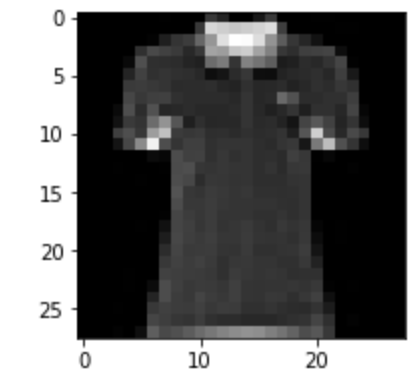
\includegraphics{label0.png}
    \caption{Shirt with corresponding label=0 "T-shirt/top"}
    \label{fig:label0}
\end{figure}

\begin{figure}[!h]
    \centering
    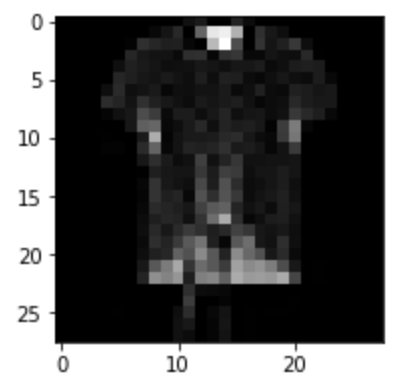
\includegraphics{label6.png}
    \caption{Shirt with corresponding label=6 "Shirt"}
    \label{fig:my_label}
\end{figure}








\section{Experiments}
\label{sec:expts}

We perform three different feature selection methods on our data. The first, which we call the "basic" feature selection is simply having each of the 784 pixel color values as an individual feature for the model. Secondly, we apply a Canny edge detection which is a multi-stage edge detector. First a Gaussian filter is applied to reduce noise in the image, and lastly edges are thinned down to a length of one pixel. The sigma parameter in the Canny filter determines the edge intensity. The Sklearn documentation provides an example image for what each step looks like. This can be seen in figure 3, where the first image has been through the Gaussian filter, and the other two images have been run through the Canny filter with differing sigma parameters. Like the basic feature selection, each of the 784 pixel values in the new image are an individual feature.

\begin{figure}[!h]
    \centering
    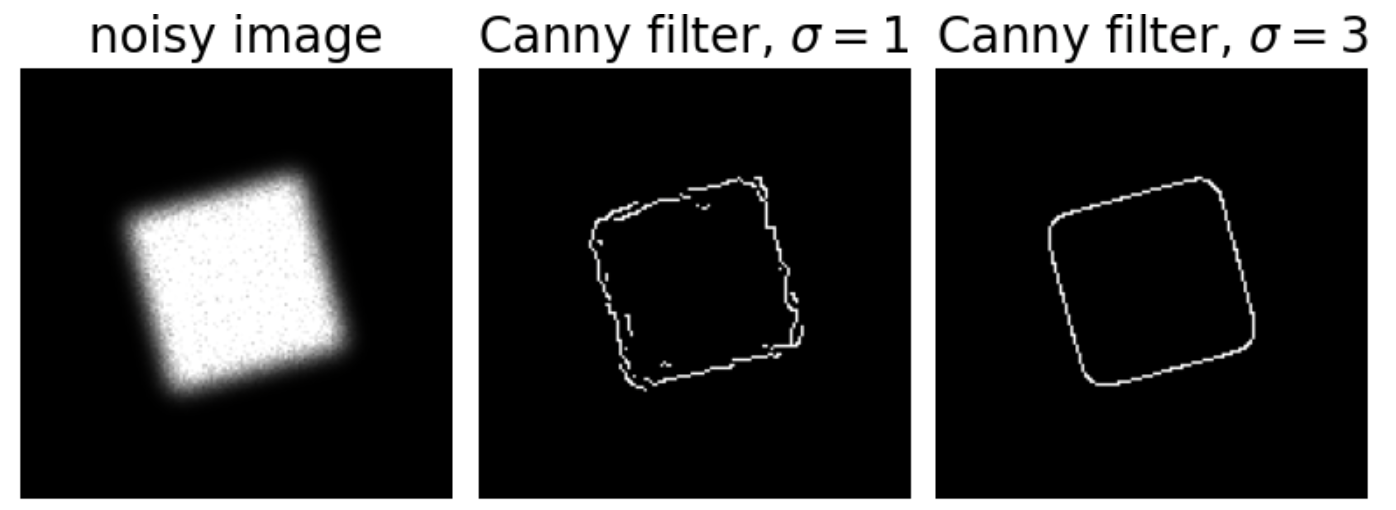
\includegraphics[width=3.33in]{canny_sklearn.png}
    \caption{Sklearn Example of Canny Filter (Source: Sklearn documentation)}
    \label{fig:my_label}
\end{figure}

In Figure 4, you can see the results of the edge detection applied to the original image with a sigma value of 1. This allows for an accurate edge detection to capture the shape of the clothing without confusing contrast in patterns/colors for edges. We expect that edge detection will reduce the noise created by different colors and patterns on the clothing and make the classification more accurate by only focusing on the general shape of each garment.

\begin{figure}[!h]
    \centering
    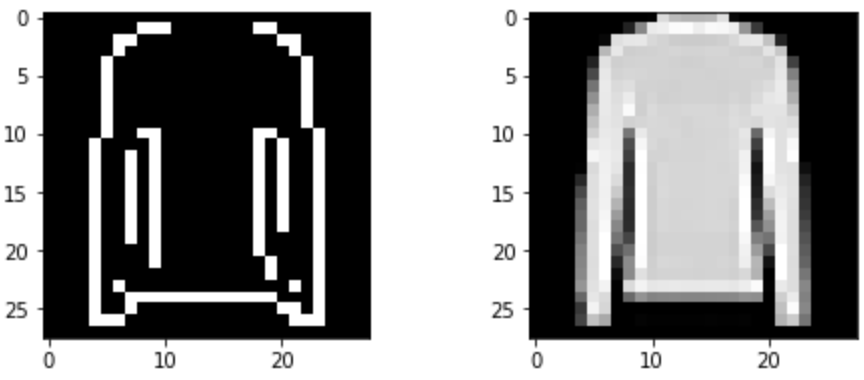
\includegraphics[width=3.33in]{canny_ex.png}
    \caption{Edge Detection (Left), Original Image (Right)}
    \label{fig:my_label}
\end{figure}

The last feature selection is a combination of the two that we are calling the "combined" feature selection. Instead of the 784 features that the basic and Canny models have, the combined model has 1568 features (784 without a filter, 784 with the filter).

Next, we run these three different sets of features through two different classification models. We use a K-nearest neighbors model (KNN) and a logistic regression model. Lastly, we created a baseline model that would always select the most common article of clothing. This provides us with a metric besides the Zhou and Bossard results to test our performance against.

Like the Zhou and Bossard paper, we used an F1 score as the measure of accuracy, as it takes into account both precision and recall by counting false negatives and false positives. Specifically we used an F1 Macro score which takes the arithmetic mean of the F1 scores for each class.

KNN classifies an input by finding the k-nearest neighbors of that given input (we use euclidean distance) and classifying that input by choosing the most common class between those k neighbors.

For the KNN model, we first tuned the value of k by using cross-validation on a smaller subset of the testing dataset (1000 images) to estimate the best value for k. We found that for the basic feature selection model, a value of $k=8$ was the most accurate on the random 1000 images. Alternatively, for the Canny and combined feature selection methods, we found that a smaller value of $k=5$ was the most accurate, as can be seen in figures 5, 6, and 7.

\begin{figure}[!h]
    \centering
    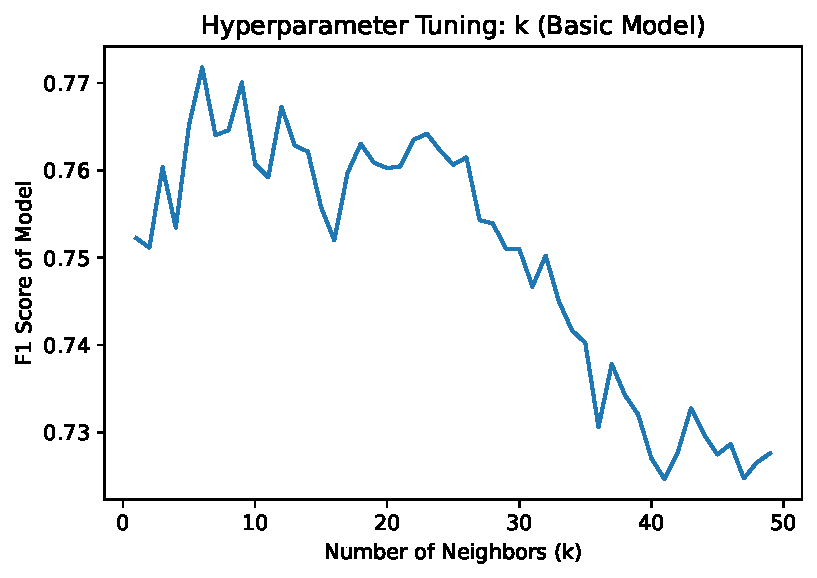
\includegraphics[width=3.3in]{tuning_k_basic.pdf}
    \caption{Basic Feature Selection Model: Tuning k}
    \label{fig:my_label}
\end{figure}

\begin{figure}[!h]
    \centering
    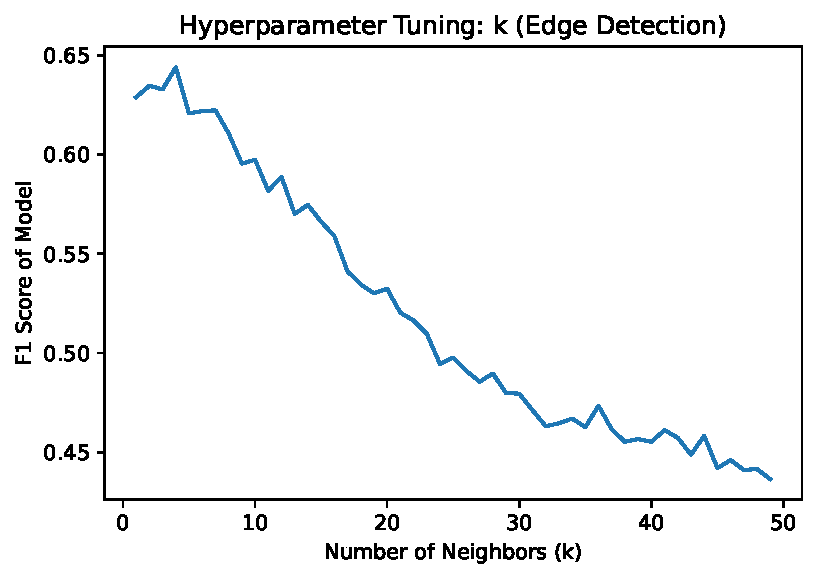
\includegraphics[width=3.3in]{tuning_k_canny.pdf}
    \caption{Canny Feature Selection Model: Tuning k}
    \label{fig:my_label}
\end{figure}

\begin{figure}[!h]
    \centering
    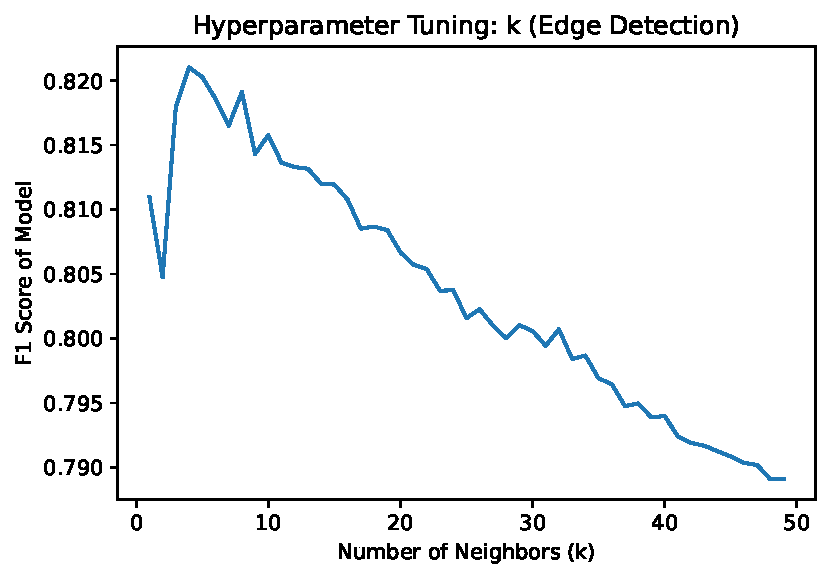
\includegraphics[width=3.3in]{tuning_k_combine.pdf}
    \caption{Combined Feature Selection Model: Tuning k}
    \label{fig:my_label}
\end{figure}

For the logistic regression, we use the "newton-cg" solver built into the sklearn library which has a more complex cost function used to enable a multi-class classification rather than the simple binary classification choice possible with the basic form of the logistic regression.

Additionally, for every model, we used cross-validation to get an idea of how accurate our models are without contaminating our testing data. It prevents us from completely over-fitting the testing data as the the intermediate accuracy measure can give an idea of how the model handles unseen data.

We expect that, for both feature selection models, either KNN or logistic regression will outperform the other for the basic, Canny, and combined feature selection methods. KNN is non-parametric and can therefore capture more complexities, and thus is more likely to overfit if the true behavior is not too complex (i.e. linear or polynomial). On the other hand, logistic regression is more likely to predict less complex behavior and therefore underfit a complex model. We assume that KNN will be better suited for a computer vision problem because each image contains many features and clothing classification is a complex problem.

\section{Results}
\label{sec:results}

The results for each feature selection model were somewhat unexpected, in that the basic model exceeded expectations. Table 2 shows the F1 scores for each model. Unsurprisingly, KNN outperforms the logistic regression for every feature selection method, as predicted. This makes sense given the complexity of the problem and the large number of features. However, the basic model outperformed the Canny model, meaning that the features of the clothing beyond just the shape was important to correctly classifying it. This also makes sense given the complexity of the problem, meaning removing features means less of the complexity is captured and biasing the model more.

\begin{table}[!h]
    \centering
    Cross Validation Results\\
    \begin{tabular}{|l|c c c|}
    \hline
         Model & Basic & Canny & Combined\\
         \hline
         Baseline & 0.018 & 0.018 & 0.018\\
         Logistic Regression & 0.783 & 0.692 & 0.783\\
         KNN & 0.856 & 0.804 & 0.855\\
         \hline
    \end{tabular}
    \caption{F1 scores for cross validation test data}
    \label{tab:my_label}
\end{table}

However, the most unexpected result was that the combined model performed equally as well as the basic model. Our guess is that the distances between color values on the basic half were much larger, giving those features a much heavier weight. This makes sense as the performance difference between both feature selection methods is essentially negligible.

Since the KNN models consistently outperformed the logistic regression models, we included confusion matrices only for the KNN models to better understand where they were making incorrect predictions. As can be seen in figures 8, 9, and 10, for all models, as predicted, the largest sources of error was mixing up the "T-shirt/top" and "Shirt" labels, and the "Coat" and "Pullover" labels. Additionally,  the "Shirt" and "Pullover" labels and the "Sneaker" and "Sandal" labels were also sources of error. This is still promising, as the model is mainly confusing similar articles of clothing rather then, for example, confusing shoes and shirts. Both the basic and combined feature selection methods had similar error distribution among categories, which further corroborates our theory above.

\begin{figure}[!h]
    \centering
    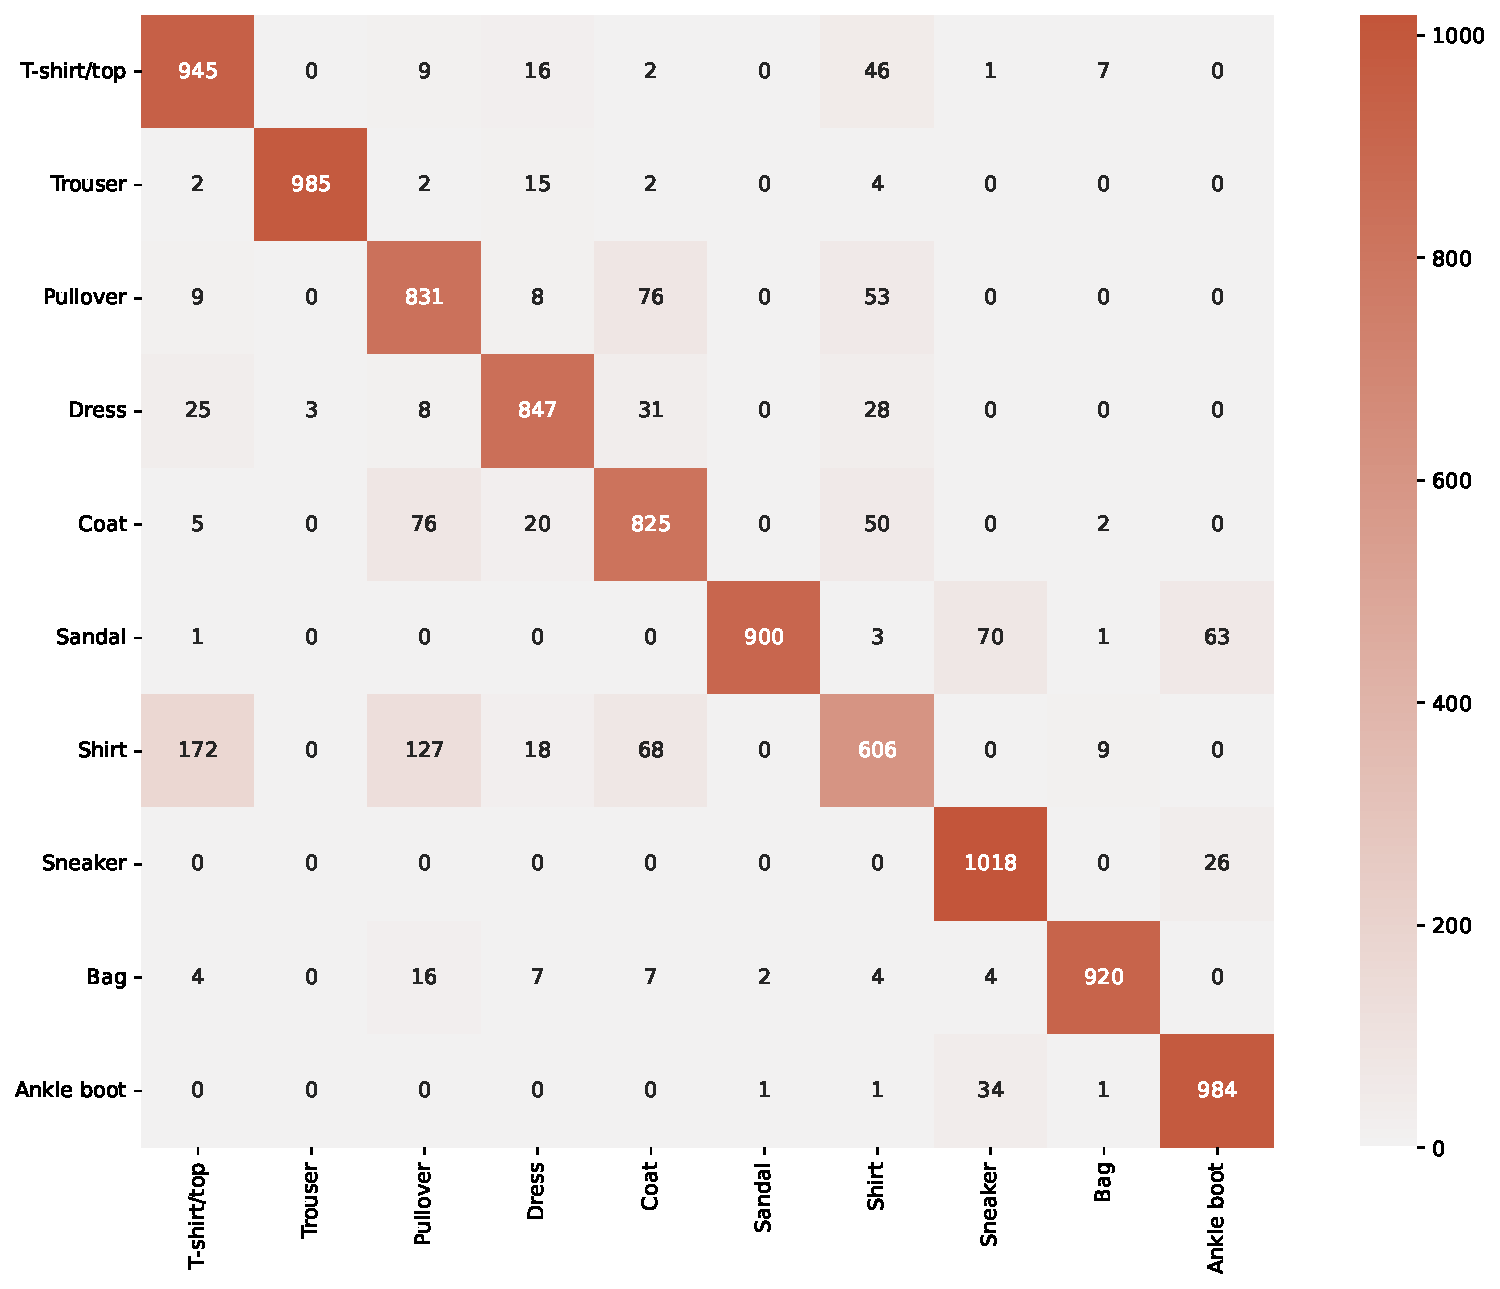
\includegraphics[width=3.5in]{basic_knn_cmatrix.pdf}
    \caption{Confusion Matrix for the basic model, predicted labels are the rows and actual labels are the columns}
    \label{fig:my_label}
\end{figure}

\begin{figure}[!h]
    \centering
    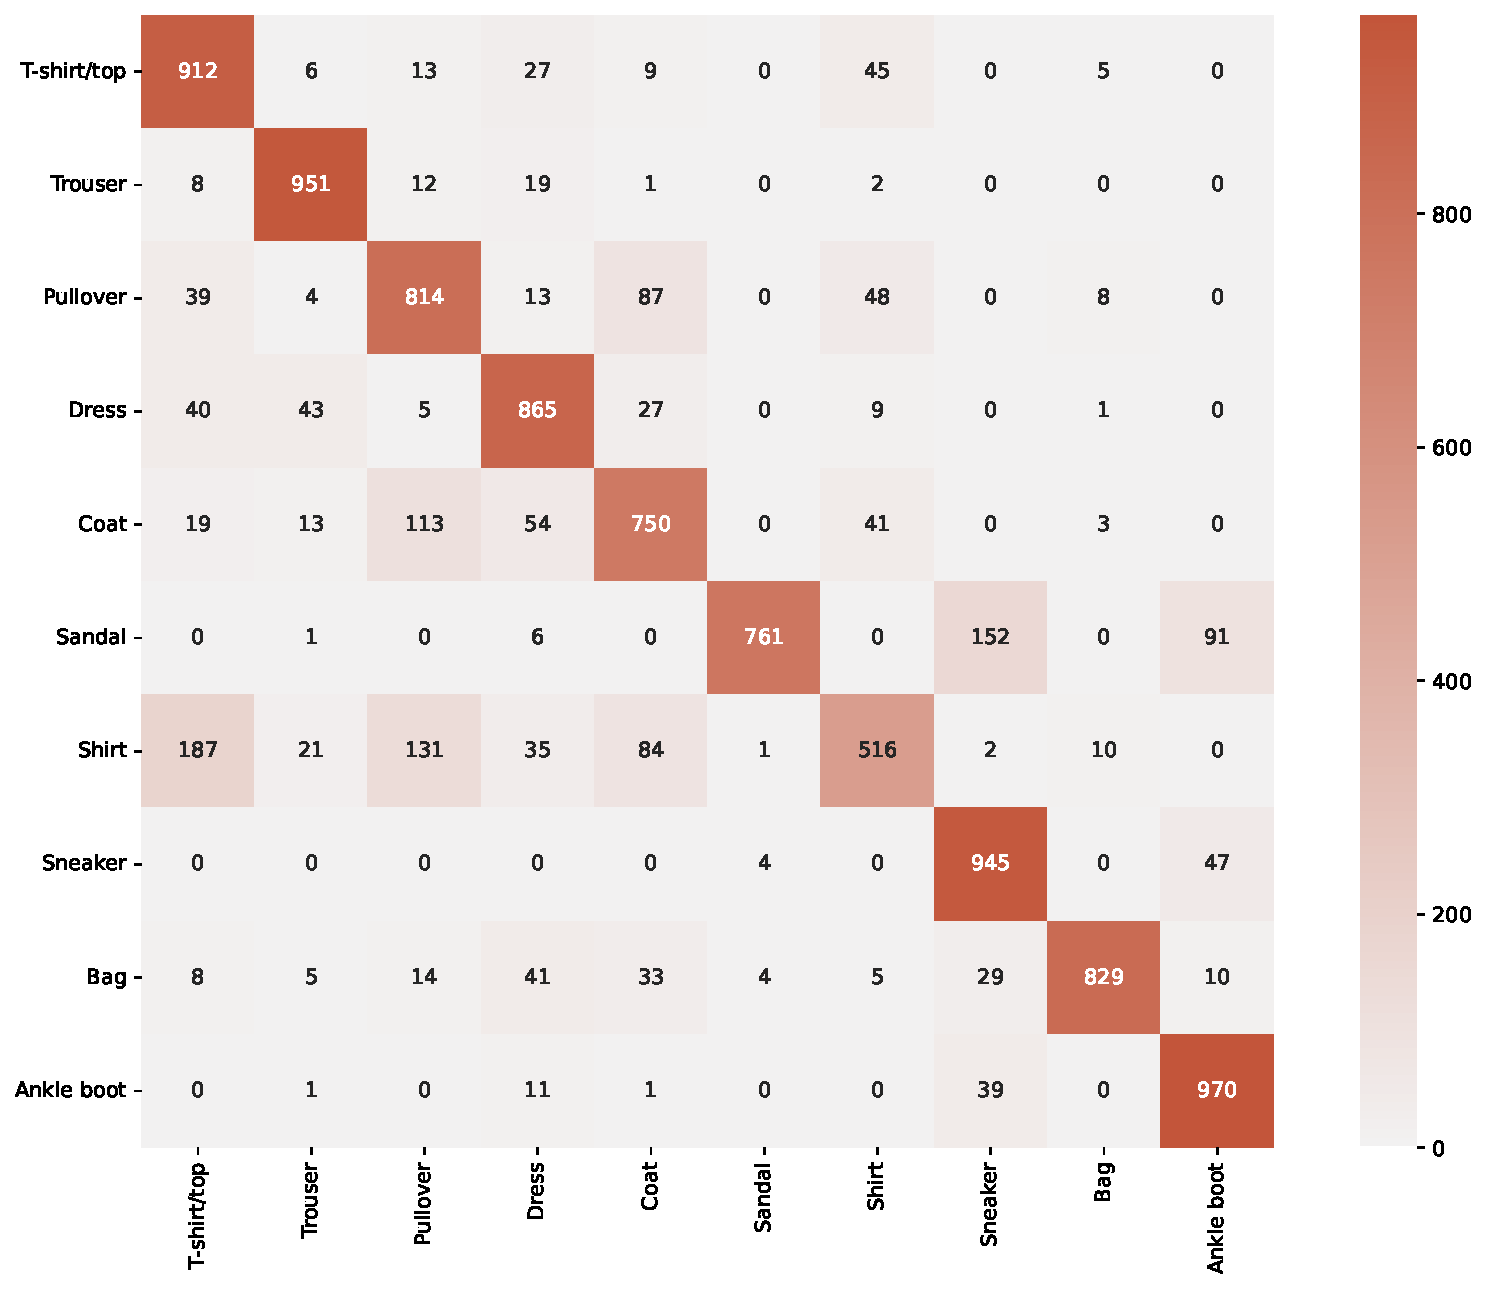
\includegraphics[width=3.5in]{canny_knn_cmatrix.pdf}
    \caption{Confusion Matrix for the Canny model, predicted labels are the rows and actual labels are the columns}
    \label{fig:my_label}
\end{figure}

\begin{figure}[!h]
    \centering
    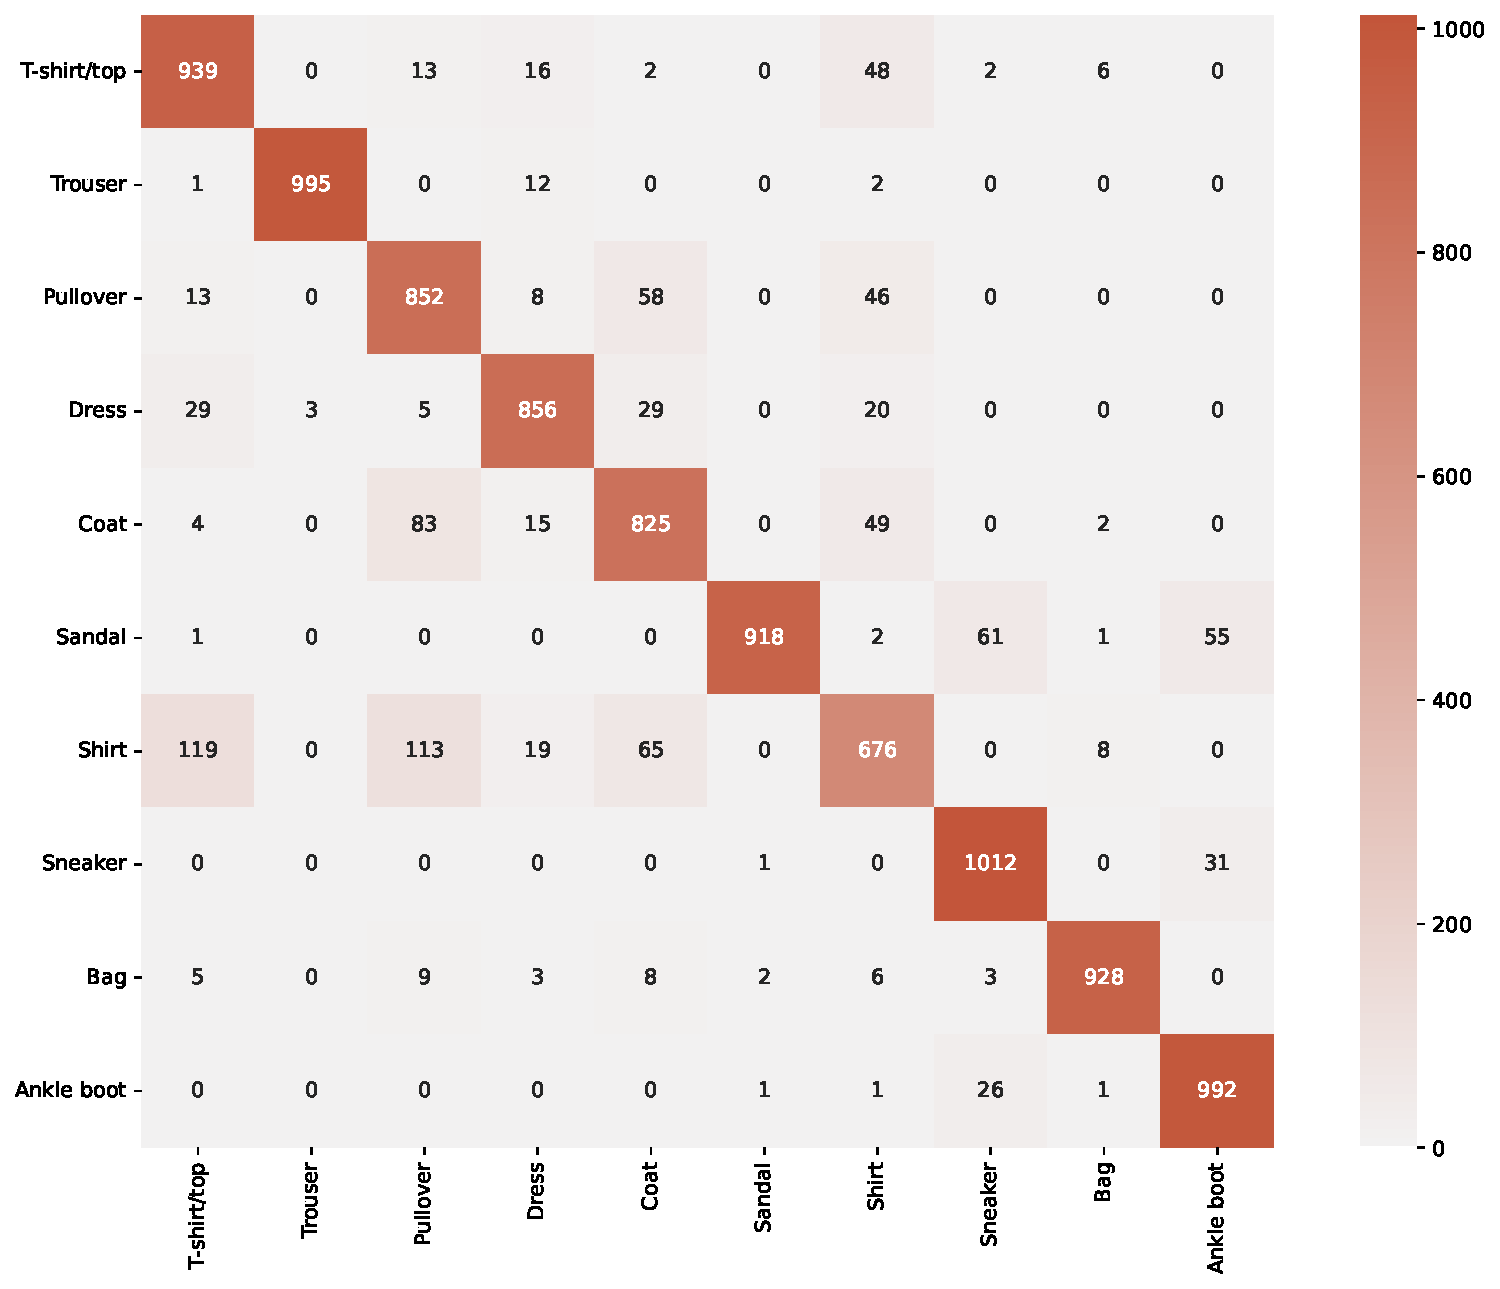
\includegraphics[width=3.5in]{combined_knn_cmatrix.pdf}
    \caption{Confusion Matrix for the combined model, predicted labels are the rows and actual labels are the columns}
    \label{fig:my_label}
\end{figure}


After tuning hyper-parameters and running the cross-validation tests, we tested the model on the final test data to get an estimate for accuracy with unseen data to see if our models overfit our training data. As displayed in table 3, most of the final test results are the same (or very similar) as the cross-validation test results-meaning the models had low variance. However, the final test score for the combined KNN model was identical to the cross-validation score, however the basic KNN model was slightly worse on the final testing data. 

\begin{table}[!h]
    \begin{center}
        Final Test Results\\
    \begin{tabular}{|l|c c c|}
    \hline
         Model & Basic & Canny & Combined\\
         \hline
         Baseline & 0.018 & 0.018 & 0.018\\
         Logistic Regression & 0.774 & 0.678 & 0.774\\
         KNN & 0.852 & 0.801 & 0.855\\
         \hline
    \end{tabular}
    \caption{F1 scores for final test data}
    \label{tab:my_label}
    \end{center}
\end{table}

This leads us to believe that the edge detection is \textit{slightly} useful in classifying clothing, as long as it is not done in isolation. Even though both the basic and combined models fit the testing data similarly, the extra edge detection features seem to create a more generally reliable model. However, the difference in F1 score of 0.003 is so slim that it is essentially negligible.

Our models all significantly outperformed our baseline model, and our KNN models even outperformed the Bossard et al. random forest model for all metrics. However, the Zhou et al. paper's use of neural networks seems to be the best approach, as their 0.93 F1 score is impressively accurate. Even though we technically outperformed the Bossard et al. paper, both papers performed the classification on images with noisy backgrounds and color, requiring more advanced feature selection techniques to isolate the important information in each image. However, for this more simplistic version of clothing classification, our model would still be useful in providing a first labeling of each article in a controlled environment, even if humans would be needed to double check images and relabel any errors.







\section{Broader Impacts}
\label{sec:impacts}

Beyond the scope of clothing classification, computer vision classification is incredibly important. It is a forefront of machine learning because it is one of the areas where humans can still outperform some models. In the most complex computer vision models, lots of feature engineering is done to capture parts of the image that humans might subconsciously understand in order to improve model accuracy, like in the Zhou et al. model.

An example of a computer vision classification problem might be classifying bird types from snapshots of natural photos, or counting the number of unique people in a photo (classifying a person as unique or seen). This could be helpful for a birding application, or automatically tracking the number of people who attend an event.

Beyond the general scope, this specific classification problem could be expanded beyond clothing to goods in general. Any type of store that needs to do some sort of inventory count (IKEA or Target or a grocery store, for example) would find an item classification problem incredibly useful to save manual classification labor. I imagine that our model would be even more useful given more distinct categories, or even classifying brand items that have more distinct colors and patterns.

\section{Conclusions}
\label{sec:concl}

Clothing classification is incredibly important for e-commerce companies or clothing brands with a digital presence. We sought to build a classification model to accurately categorize articles of clothing given an image. We used each pixel of the image as a feature as well as applying a Canny edge detection filter to extract more features. We tested a k-nearest-neighbors (KNN) approach as well as a logistic regression, and found that the KNN model was more accurate across our different feature selection methods.

Furthermore, we found that a KNN model using a combined feature selection strategy of concatenating two images, one with basic unfiltered color values for each pixel and the other being the original image with a Canny edge detector applied. We found that this method was slightly more accurate than the basic color values alone. 

One way that we think we can improve this model is by applying even more robust feature selection methods. The Zhou et al. paper trains a neural network to extract features from their image, which they believe was effective in boosting accuracy. This would be much more complex, but would most likely boost our model's accuracy. Additionally, our model would be much better if we edited the labels to remove ambiguity and distinguish categories better. Additionally, higher definition images would help to better distinguish small differences in each image.


% This creates the references section. Open the project1.bib file to
% see how to organize your references.
\bibliography{project1}
\bibliographystyle{aaai} % sets citation and bib style, do not modify

\end{document}
